\chapter{Temporal Depth Smoother}
\label{cha:smoother}

A learned post-processing stage between depth inference and data processing removes temporal
flicker from inferred depth.

\section{Motivation}
\label{sec:smoother-motivation}

Depth inference (Chapter~\ref{cha:system-design}) runs a geometry model per frame on ``fake''
sliding-window input. Its depth is temporally unstable. Surfaces that do not move change depth from
one frame to the next, and the object--background and object--controller boundaries shift, so the
silhouette moves while the object itself is still. Since 2D correspondences are lifted into 3D with
these values, that jitter reaches the tracked points, the reconstruction, and the warp model.

Video depth models such as \textcite{vda} are smooth, but they are geometrically weak and monocular,
so they do not suit a multi-camera capture (see the results comparison in Table~\ref{tab:app-vid-variants}, Appendix~\ref{app:results}). Earlier stabilisation work either couples to a specific
depth backbone \parencite{nvds,nvdsp} or assumes labelled sensor ground truth
\parencite{stabledpt,li2023consistent}. The stage described here has to meet a narrower requirement:
it must apply to any flickering depth sequence, need no ground truth, and work across views.

\section{Learning a Residual Correction}
\label{sec:smoother-idea}

The two model families fail in opposite places: the geometry model has good \emph{spatial}
structure, and the video model has good \emph{temporal} structure. Depth and RGB are encoded into a
latent space and decoded into a smooth prediction, which is scored by temporal penalties taken from
the video model and geometric penalties taken from the geometry model.

Rather than predict a depth map, the network predicts a \emph{residual} that is added to the geometry
model's prediction. The video model serves as a motion oracle, not a depth reference: its values are
relative, so no metric scale is inherited from it.

\section{Architecture}
\label{sec:smoother-architecture}

\begin{figure}[H]
	\begin{center}
		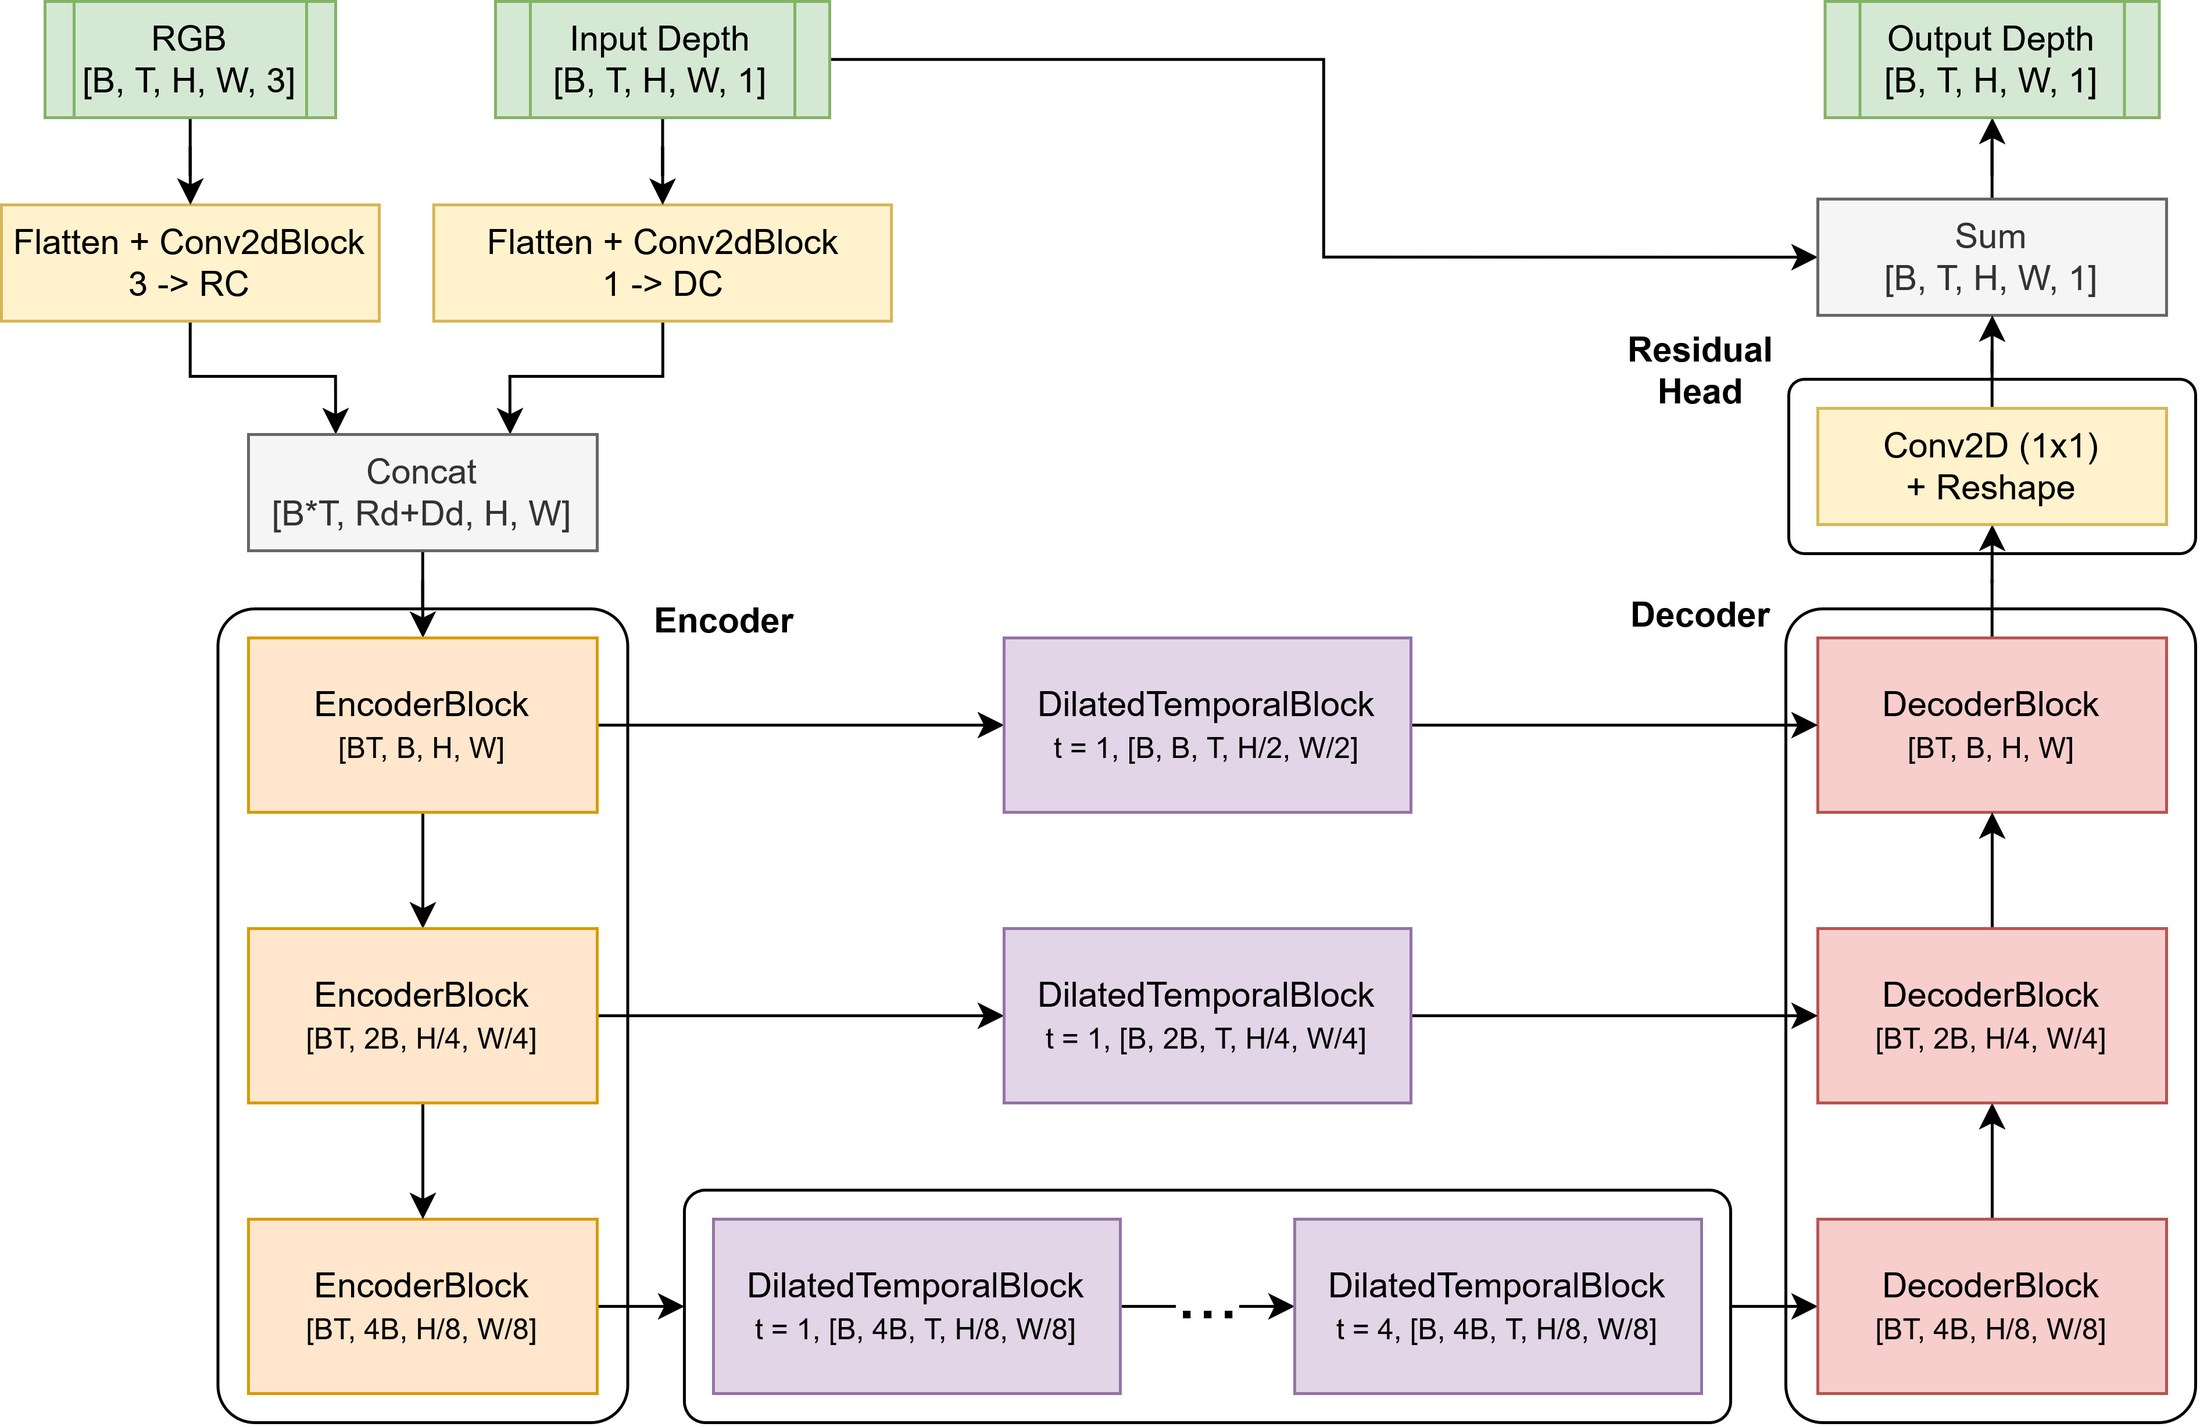
\includegraphics[width = 0.9\textwidth]{Images/smoother_architecture}
		\caption{The temporally-dilated residual U-Net.}
		\label{fig:smoother-architecture}
	\end{center}
\end{figure}

The network has to learn and preserve structure from the geometry model, absorb temporal consistency
from the video model, and correct each frame using both depth maps and the RGB image. A diffusion-
or DPT-style backbone was considered and rejected, because it was deemed overkill and potentially too expensive. The chosen design is a small 4.7-million-parameter \textbf{temporally-dilated residual U-Net}.
Spatial structure is preserved across scales, and temporal dilation gives each frame context from
several time offsets without processing the whole clip. Its size is limited by the training compute
available.

The U-Net is assembled from four blocks (Figure~\ref{fig:smoother-blocks}). The per-frame 2D block,
\texttt{Conv2dBlock}, is two $3\times3$ convolutions, each followed by GroupNorm and ReLU. An
\texttt{EncoderBlock} runs one of these and taps the skip connection before a strided $2\times2$
convolution halves the resolution. A \texttt{DecoderBlock} doubles the resolution with a transposed
convolution, concatenates the matching skip and refines the result with a \texttt{Conv2dBlock}; a
learned upsample is used because bilinear upsampling produced smearing and edge artefacts. The
\texttt{DilatedTemporalBlock} is a single $3\times3\times3$ convolution, dilated only in time, with
GroupNorm, ReLU and a residual connection. Stacking dilations $1, 2, 4, 8$ at the bottleneck gives
each output frame a receptive field of $\pm15$ frames; shallower levels use dilation 1.

\begin{figure}[H]
	\begin{center}
		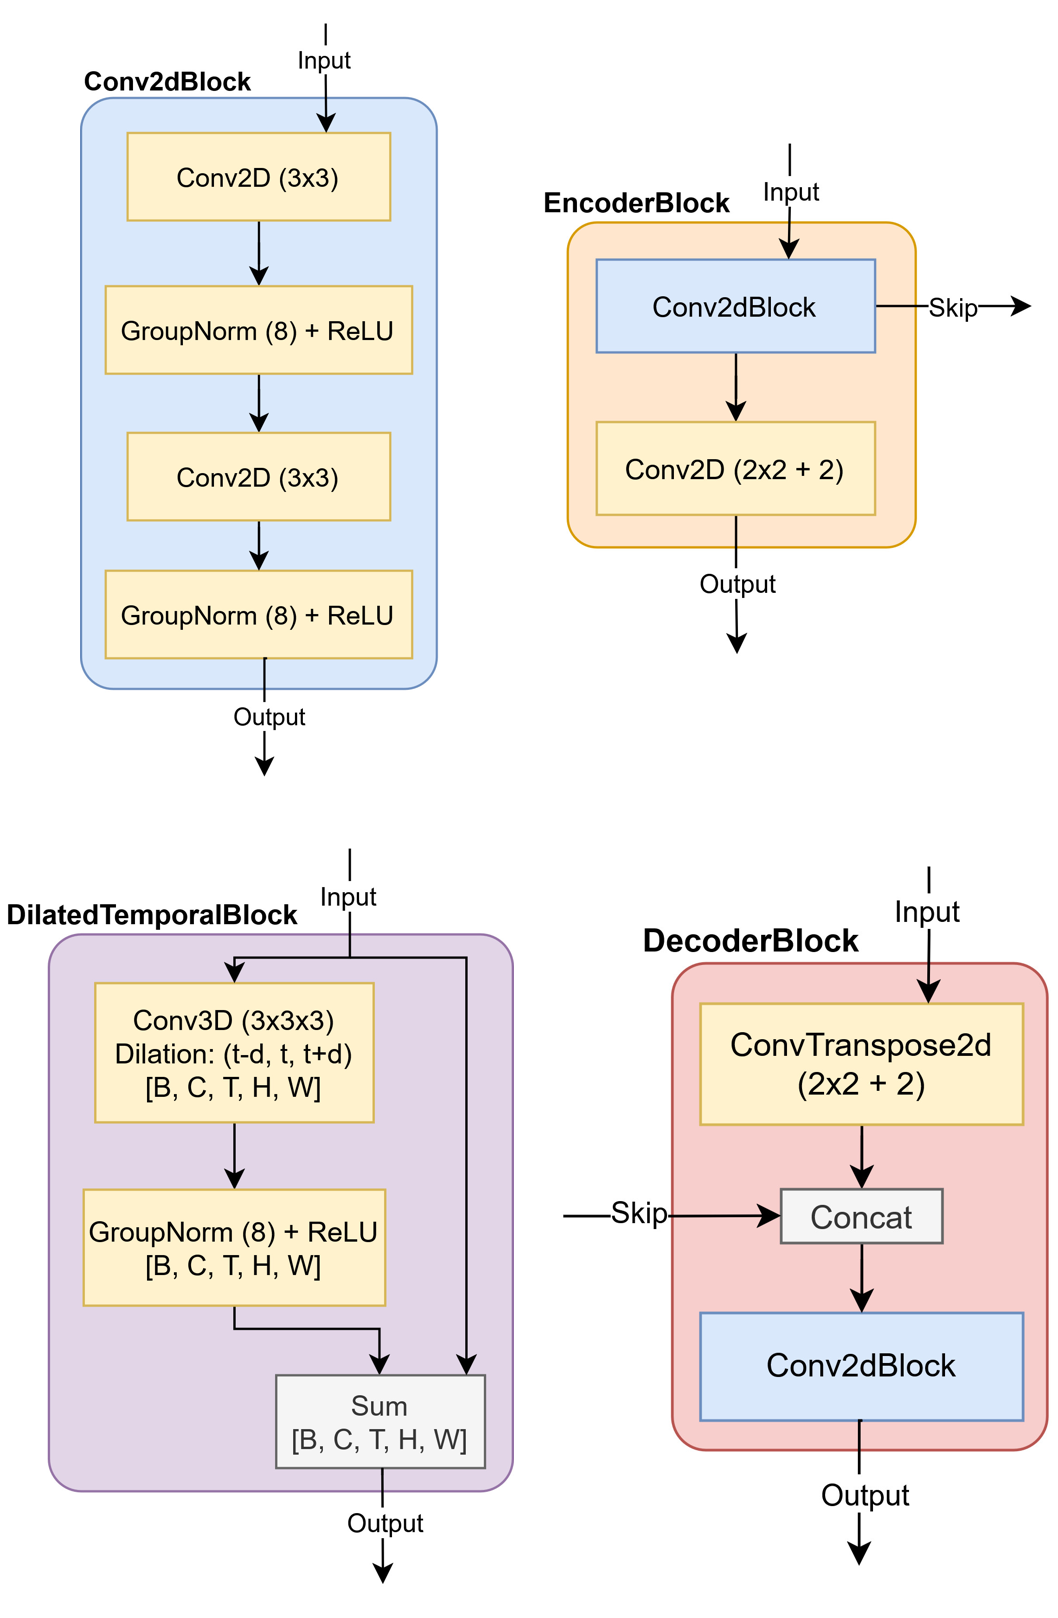
\includegraphics[width = 0.8\textwidth]{Images/block_grid}
		\caption{The four building blocks of the smoother, drawn to a common scale:
		(a)~\texttt{Conv2dBlock}, (b)~\texttt{EncoderBlock}, (c)~\texttt{DilatedTemporalBlock} and
		(d)~\texttt{DecoderBlock}, which reinserts the skip connection that the encoder taps.}
		\label{fig:smoother-blocks}
	\end{center}
\end{figure}


\section{Loss Functions}
\label{sec:smoother-losses}

The objective combines fidelity, temporal gradient matching (TGM), temporal total variation (TV),
and two geometric penalties: edge sharpness and spatial-gradient matching. 

Let $D^s$, $D^0$ and $D^v$ denote the smoothed output, raw DA3 depth and aligned VDA depth. For
frame skip $k$, define
\[
    \Delta_k D_{b,t,x}=D_{b,t+k,x}-D_{b,t,x},\qquad
    \Delta_k^2D_{b,t,x}=D_{b,t+2k,x}-2D_{b,t+k,x}+D_{b,t,x}.
\]
Here $b$ indexes a clip, $t$ a frame and $x$ a pixel. Angle brackets denote a mean over valid
clips, frame indices and pixels. Denominators are clamped below by $\epsilon=10^{-6}$. The equations follow the implementation.

\paragraph{Temporal gradient matching loss.}
\label{sec:smoother-tgm}

For each span $k$, TGM matches temporal depth differences to VDA. The VDA values provide a motion
signal, not a depth target. Each span is normalised by the discrepancy between raw DA3 and VDA:
\[
    B_{\mathrm{tgm}}^{(k)}
      =\max\!\left(\left\langle\left|\Delta_kD^0-\Delta_kD^v\right|\right\rangle,\epsilon\right),
    \qquad
    \mathcal{L}_{\mathrm{tgm}}^{(k)}
      =\frac{\left\langle\left|\Delta_kD^s-\Delta_kD^v\right|\right\rangle}
                  {B_{\mathrm{tgm}}^{(k)}}.
\]
The implementation combines $k=1,2,3$ as
\[
    \mathcal{L}_{\mathrm{tgm}}
      =\mathcal{L}_{\mathrm{tgm}}^{(1)}
       +0.25\,\mathcal{L}_{\mathrm{tgm}}^{(2)}
       +0.07\,\mathcal{L}_{\mathrm{tgm}}^{(3)}.
\]
Larger skips capture slower oscillations; their weights are code defaults and have not been
systematically tuned.


\paragraph{Temporal total variation loss.}
\label{sec:smoother-tv}

TV penalises the output's second temporal difference. VDA acceleration gates the penalty, reducing
it where the motion oracle reports acceleration. For each span,
\[
    w_{b,t,x}^{(k)}
      =\exp\!\left(-10\left|\Delta_k^2D^v_{b,t,x}\right|\right),
    \qquad
    B_{\mathrm{tv}}^{(k)}
      =\max\!\left(\left\langle\left|\Delta_k^2D^0\right|w^{(k)}\right\rangle,\epsilon\right),
\]
\[
    \mathcal{L}_{\mathrm{tv}}^{(k)}
      =\frac{\left\langle\left|\Delta_k^2D^s\right|w^{(k)}\right\rangle}
                  {B_{\mathrm{tv}}^{(k)}},
    \qquad
    \mathcal{L}_{\mathrm{tv}}
      =\mathcal{L}_{\mathrm{tv}}^{(1)}+0.25\,\mathcal{L}_{\mathrm{tv}}^{(2)}.
\]
The exponential constant and span weights come from the implementation and were not tuned.


\paragraph{Fidelity loss.}
\label{sec:smoother-fidelity}

Fidelity keeps the output close to DA3 in a shared, clip-level scale. Let $m_{b,x}=\operatorname{median}_tD^0_{b,t,x}$,
$t_b=\operatorname{median}_x m_{b,x}$ and
$s_b=\max(\operatorname{mean}_x|m_{b,x}-t_b|,\epsilon)$. The aligned depth is
$A_b(D)=(D-t_b)/s_b$. For the VDA gate, let
$\mu_v=\langle|\Delta_1D^v|\rangle+\epsilon$ and $\gamma=0.25$:
\[
    g_{b,0,x}=1,\qquad
    g_{b,t,x}=\gamma+(1-\gamma)
       \exp\!\left(-\frac{|\Delta_1D^v_{b,t-1,x}|}{\mu_v}\right),\quad t>0,
\]
\[
    B_{\mathrm{fid}}=\max\!\left(\operatorname{std}(A(D^0)),\epsilon\right),
    \qquad
    \mathcal{L}_{\mathrm{fid}}
      =\frac{\left\langle g\,|A(D^s)-A(D^0)|\right\rangle}{B_{\mathrm{fid}}}.
\]
The gate is strongest in temporally stable regions and relaxes toward $0.25$ where VDA reports
motion. Its scale and location statistics are computed from DA3, not VDA.


\paragraph{Geometric loss.}
\label{sec:smoother-geometric}

The implementation has two spatial penalties. Define forward finite differences by
$\nabla_xD_{b,t,i,j}=D_{b,t,i,j+1}-D_{b,t,i,j}$ and
$\nabla_yD_{b,t,i,j}=D_{b,t,i+1,j}-D_{b,t,i,j}$, padding the last column and row with zero.
The edge-sharpness penalty uses Sobel magnitudes $G(I)$ of grayscale RGB and $G(D^v)$ of VDA
depth, each divided by its per-clip 95th percentile. It keeps pixels identified as edges in both
signals and penalises smoothed edges below $0.8$ of the VDA edge magnitude:
\[
    M=\mathbf{1}[\widetilde G(I)>0.6]\,\mathbf{1}[\widetilde G(D^v)>0.6],\qquad
    \mathcal{L}_{\mathrm{edge}}
      =\frac{\operatorname{mean}_{M=1}
             [\,0.8\widetilde G(D^v)-\widetilde G(D^s)\,]_+}
             {\max\!\left(\operatorname{mean}_{M=1}\widetilde G(D^v),\epsilon\right)}.
\]
Here $[q]_+=\max(q,0)$; an empty mask gives zero numerator. The second penalty compares forward
finite-difference gradients of smoothed and raw DA3 depth, weighted by VDA Sobel magnitude. With
$W=\max(0.1,G(D^v)/(\operatorname{mean}_{t,x}G(D^v)+\epsilon))$,
\[
    \mathcal{L}_{\mathrm{grad}}
      =\frac{\frac12\sum_{a\in\{x,y\}}\left\langle W\,
             |\nabla_aD^s-\nabla_aD^0|\right\rangle}
             {\max\!\left(\frac12\sum_{a\in\{x,y\}}\left\langle W|\nabla_aD^0|\right\rangle,
             \epsilon\right)}.
\]
Both spatial terms are baseline-normalised in the implementation. Their individual effects have
not been isolated in the evaluation.


\paragraph{Combined objective.}
\label{sec:smoother-combined}

The weighted objective is
\[
    \mathcal{L}
      =\lambda_{\mathrm{fid}}\mathcal{L}_{\mathrm{fid}}
       +\lambda_{\mathrm{tgm}}\mathcal{L}_{\mathrm{tgm}}
       +\lambda_{\mathrm{tv}}\mathcal{L}_{\mathrm{tv}}
       +\lambda_{\mathrm{edge}}\mathcal{L}_{\mathrm{edge}}
       +\lambda_{\mathrm{grad}}\mathcal{L}_{\mathrm{grad}}.
\]
The training configuration gives $\lambda_{\mathrm{fid}}=1.3$, $\lambda_{\mathrm{tgm}}=0.8$,
$\lambda_{\mathrm{tv}}=0.8$, $\lambda_{\mathrm{edge}}=0.05$ and
$\lambda_{\mathrm{grad}}=0.04$. The span weights are listed in Appendix~\ref{app:hyperparameters}. These settings remain untuned.


\section{Training}
\label{sec:smoother-training}

The training run uses 162 complete clip-camera inputs and saves a
best-model checkpoint. The deterministic split is by clip, so frames from a validation clip do not
enter training. Table~\ref{tab:smoother-training} records the training configuration.

\begin{table}[H]
    \caption{Temporal smoother training configuration.}
    \label{tab:smoother-training}
    \begin{center}
        \begin{tabular}{@{}p{3.6cm}p{10.4cm}@{}}
            \toprule
            Setting & Recorded value \\
            \midrule
            Complete clips & 162 clip-camera inputs; 130 train and 32 validation (80:20, seed 42, split by clip) \\
            Training samples & 1,842 windows; length 16 frames, stride 8 \\
            Validation samples & 264 windows; length 16 frames, stride 16 \\
            Input size & $226\times334$ pixels; RGB and depth are resized \\
            Batch and workers & Batch size 2; 2 data-loader workers \\
            Optimiser & Adam; weight decay $10^{-4}$ \\
            Learning rate & $3\times10^{-3}$; ReduceLROnPlateau, factor $0.5$, patience 5 \\
            Duration & 50 epochs; checkpoints saved for each epoch \\
            Precision & CUDA autocast with bfloat16 enabled \\
            Loss weights and temporal spans & See Table~\ref{tab:app-lossweights} (Appendix~\ref{app:hyperparameters}) \\

            Augmentation and hardware & No augmentation in the loader; NVIDIA GeForce RTX 3060 \\
            \bottomrule
        \end{tabular}
    \end{center}
\end{table}

Training ran on a single NVIDIA GeForce RTX 3060. The loader resizes and normalises inputs but
applies no augmentation.


\section{Inference}
\label{sec:smoother-inference}

Inference follows the video model. Clips are processed in overlapping chunks, which provides
temporal context without holding an entire sequence in memory; the chunks are blended with the
weighted window of Figure~\ref{fig:smoother-inference}. Resolutions are arbitrary with minimal
padding, and depth maps are never resized, since resizing would destroy the sub-pixel frame-to-frame
consistency the stage exists to produce.

\begin{figure}[H]
	\begin{center}
		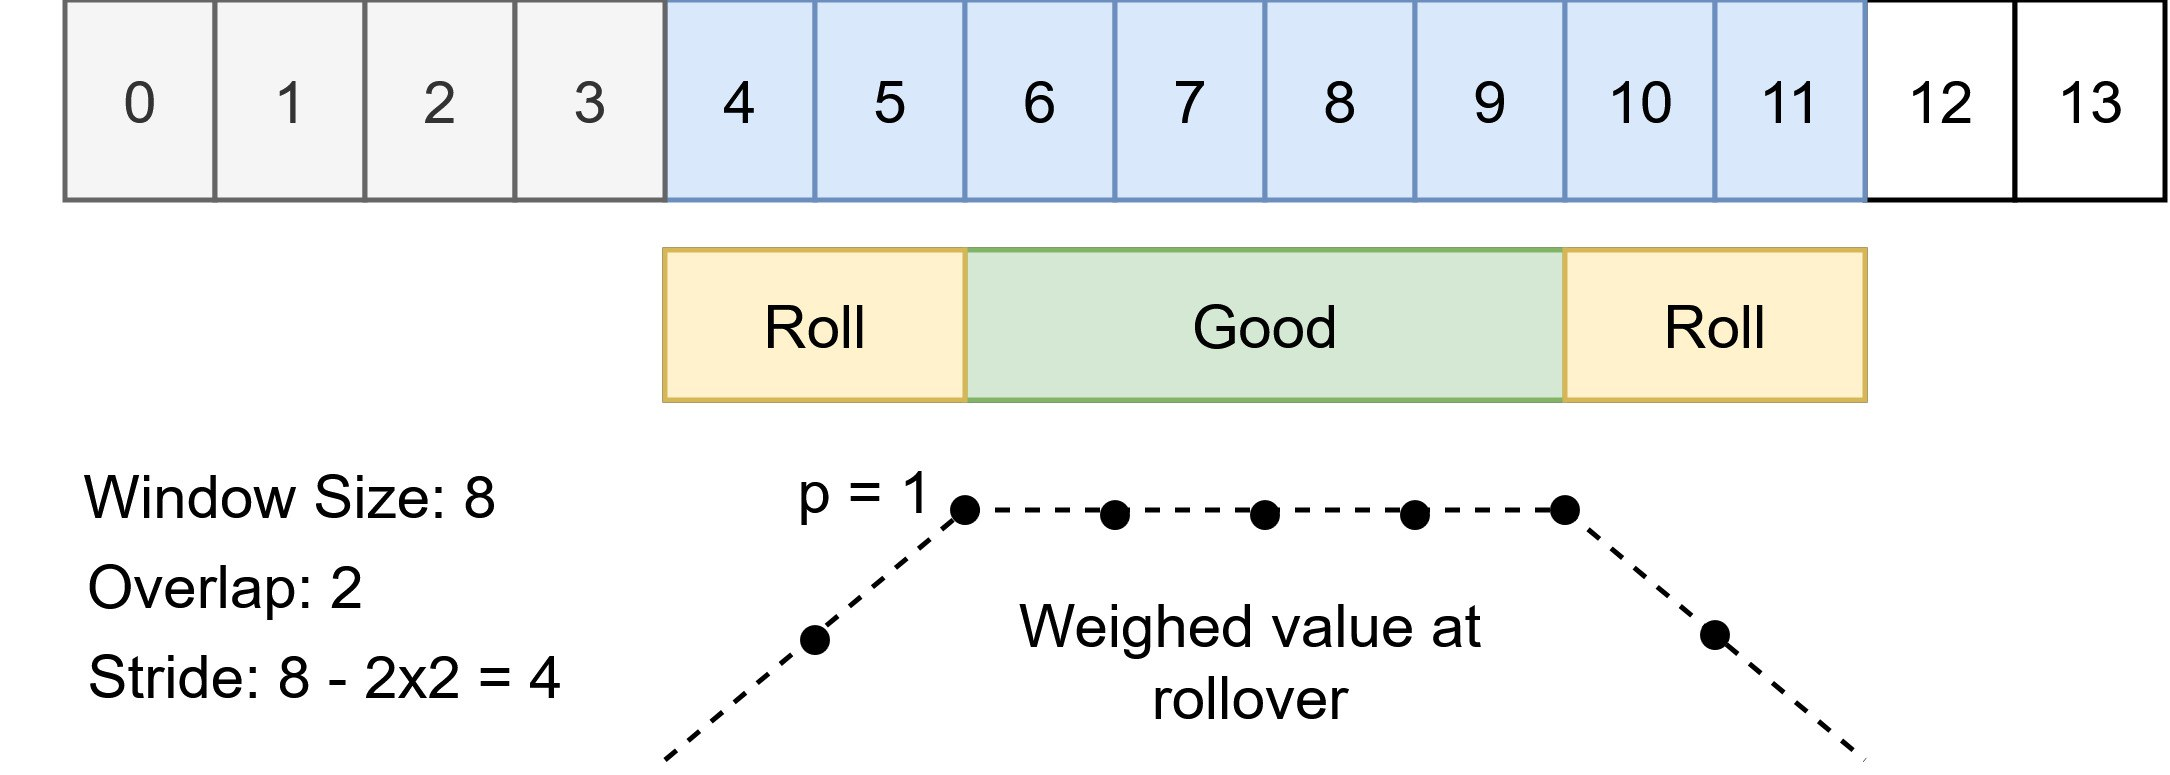
\includegraphics[width = \textwidth]{Images/smoother_inference}
		\caption{Weighted sliding-window inference. Overlapping chunks are blended into one output
		sequence.}
		\label{fig:smoother-inference}
	\end{center}
\end{figure}

Figure~\ref{fig:smoother-beforeafter} shows four frames, two each from a mat lift and a sloth
stretch, before and after smoothing with the best saved model. Consecutive-frame comparisons over
five sequences are shown in Figure~\ref{fig:eval-depth-cases} (Chapter~\ref{cha:evaluation});
full recorded clips are listed in Appendix~\ref{app:results}.

\begin{figure}[H]
	\begin{center}
		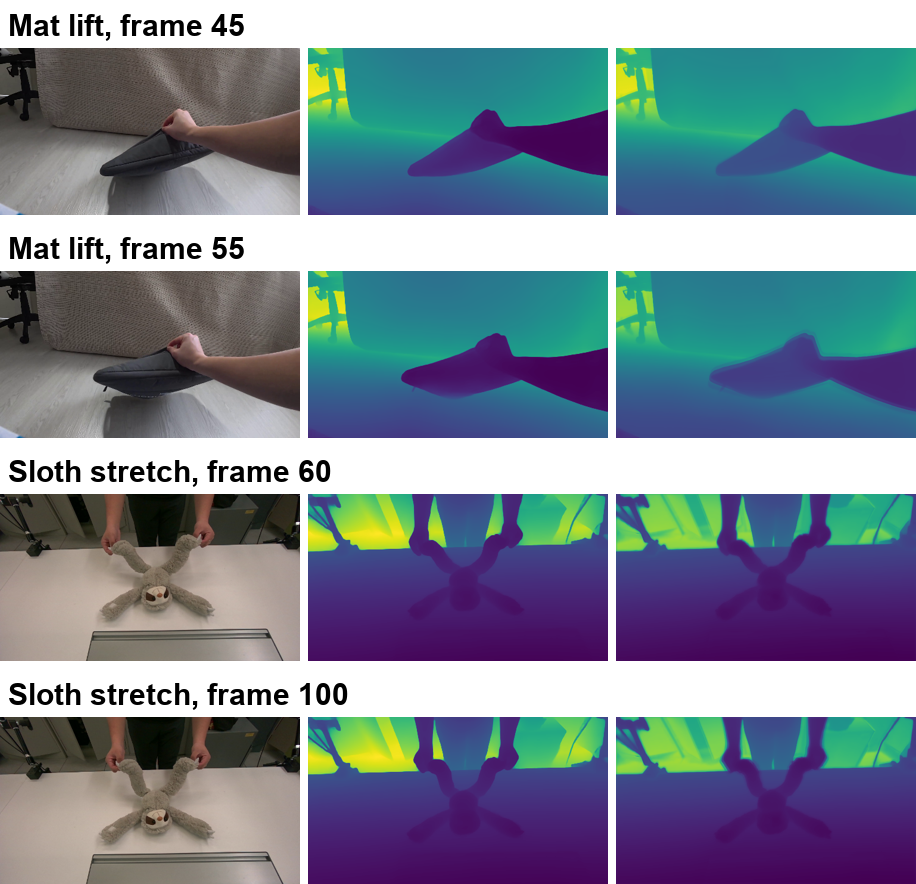
\includegraphics[width = \textwidth]{Images/smoother_beforeafter}
		\caption{RGB input, raw DA3 depth and smoothed depth for four frames of a mat-lift and a
		sloth-stretch sequence.}
		\label{fig:smoother-beforeafter}
	\end{center}
\end{figure}


\section{Properties and Limitations}
\label{sec:smoother-properties}

The stage can be reused independently of this project:

\begin{enumerate}
	\item It applies to any flickering depth map, because it predicts a correction and needs no
	      specific backbone.
	\item It requires no ground-truth depth and no labelled dataset.
	\item It handles arbitrary resolutions without resizing.
	\item It is small and fast relative to the depth model it corrects.
\end{enumerate}

Some limitations remain. Smoothing visibly blurs depth, and there is not enough evidence that the
correction targets object flicker vs stationary flicker. The hyper-parameters are untuned, and the
results depend heavily on these settings. The stage has not been validated on other depth backbones, and it is not clear how well it generalises to other domains.
